\documentclass[12pt]{article}

%% preamble: Keep it clean; only include those you need

% if the below packages cannot be installed automatically, you can 
% download the required .sty files from CTAN and place them in the
% same location as the .tex file (or upload to overleaf in same
% location (folder) in overleaf

\usepackage{amsmath}
\usepackage[margin = 1in]{geometry}
\usepackage{graphicx}
\usepackage{booktabs}
\usepackage{natbib}

\usepackage{lineno}  % use these two lines to include line numbers
\linenumbers

\usepackage{setspace} % for doublespacing
\doublespacing


% highlighting hyper links
\usepackage[colorlinks=true, citecolor=blue]{hyperref}


\usepackage{color}
\newcommand{\blue}{\color{blue}} 
% when you make your edits in response to review/instructor comments, 
% you can indicate changes in color

%% meta data

\title{A concise meaningful title}
\author{Elizabeth Schifano\\
  Department of Statistics\\
  University of Connecticut
}

\begin{document}
\maketitle

\begin{abstract}
Here is the abstract.  
Avoid notations; avoid citations; generally should not exceeding 250 words. 
Consult Note 5 on the STAT4916W course website for specific information about 
what should be included in this section and others.  Also remember the general 
\LaTeX\mbox{ } guidelines and tips from STAT4916W Note 2. 
Include keywords at the end of the abstract section; they should be 
alphabetized and not repeat any words in the title.\\

\noindent\textbf{Keywords}: keyword1, keyword2, keyword3.
\end{abstract}


\section{Introduction}
\label{sec:intro}

The introduction needs to answer three questions to provide context and 
relevance:
\begin{enumerate}
\item Why should we care about this research (its importance)?
\item What has been done in the literature (identify a gap)?
\item What is new (your contributions)?
\end{enumerate}


When citing literature, be sure to understand the difference of
textual citations and parenthetical citations.  Here are some examples. 

\citet{xie2015dynamic} did something ...  


Recently there has been an increase in the prevalence of diabetes in the United 
States \citep{wild2004global}. Notice that the citation is included 
\textit{inside} the punctuation, as it is part of the sentence. 


Considerable work has already been published in this area 
\citep[e.g.,][]{xie2015dynamic}. Some parametric bootstrap sample size 
approach was proposed by \citet{dwivedi2017analysis}. 


Also notice the use of \verb|\label|-\verb|\ref| pairing within the source 
(.tex) document to enable cross-referencing of sections, tables, and figures.


The next paragraph is a roadmap for the rest of your manuscript.  The
roadmap paragraph should be the final paragraph in Section~\ref{sec:intro}.
Notice in the previous sentence that the 'S' in section is capitalized when we 
refer to a specific numbered section. Similarly the 'T' in table and
'F' in figure should be capitalized when referring to specific numbered tables 
and figures (see examples in Sections~\ref{sec:data} and~\ref{sec:resu}).


The rest of the paper is organized as follows. The data will be presented in 
Section~\ref{sec:data}. Section~\ref{sec:meth} describes the methods. The 
results are reported in Section~\ref{sec:resu}. A discussion concludes in 
Section~\ref{sec:disc}.  



\section{Data Description}
\label{sec:data}

Use this section to describe the data that helps to answer your research
questions. Some descriptive statistics in tables or figures are suggested 
here to summarize data.  See Notes 4 and 5 for details.


The response variable $Y$ is the log-concentration of calcium in the blood, 
measured in mg/dL. Notice that we use \$ to enclose display-math expressions, 
including just variable names.   


Each table and figure included must be explicitly referenced and commented upon
in the text.  For example, Table~\ref{tab:rv} summarizes some distributional 
features for some of the variables in our dataset. The \verb|[!t]| specification 
forces the table to be located at the top of the page. 

\begin{table}[!t]
  \caption{This is my first table.  Table captions should be located above the
	table.}
	\label{tab:rv}
\centering
\begin{tabular}{lrrr}
  \toprule
& Var 1 & Var 2 & Var 3 \\ 
  \midrule
Feature 1 & $-$0.110 & 4 & 2.401 \\ 
Feature 2 &    0.116 & 4 & 3.529 \\ 
Feature 3 & $-$0.066 & 6 & 11.104 \\ 
Feature 4 &    0.219 & 3 & 4.815 \\ 
Feature 5 &    0.303 & 5 & 2.188 \\ 
Feature 6 &    0.544 & 0 & 8.050 \\ 
Feature 7 & $-$2.617 & 8 & 3.646 \\ 
  \bottomrule
\end{tabular}
\end{table}


\section{Methods}
\label{sec:meth}

Use this section to present the methodologies that will generate results by
analyzing the data. Only the methods should be described in this section; the 
results go in the next section.  

It is strongly advised \textbf{NOT} to combine Methods and Results into one 
section.  


\subsection{First Subheading}

It may be wise to break up Section~\ref{sec:meth} into multiple subsections.
Remember that good headings and subheadings are not only helpful when first
organizing our thoughts and starting the first draft, but are also helpful in 
orienting the reader to the structure of the report.  For example, feature 
selection, model selection and training, and evaluation metrics may be great subheadings.  


{\blue This text is in blue. It is sometimes helpful to highlight (in color) the 
changes that were made in response to reviewer's comments.}


\subsection{Some Equation Examples}

Recall Einstein's equation
\begin{equation}
  \label{eq:mc2}
  E = m c^2,
\end{equation}
which states that the energy $E$ of a particle in its rest frame as the product
of mass ($m$) with the speed of light squared ($c^2$). Equation~\eqref{eq:mc2} 
is a display-math expression.


Suppose that the radius of a circle is $r$. Then its area is given by
\begin{equation}
  \label{eq:area}
   \pi r^2.
\end{equation}
%
Equation~\eqref{eq:area} is interesting, although it is short. If the expression 
is not referenced elsewhere in the document, would likely be better as an inline 
expression, as in `Then its area is given by $\pi r^2$.' 


We can avoid numbering (labeling) a display-math expression by enclosing the 
expression with \verb|\[| and \verb|\]|, as in
\[
  f(x) = \frac{1}{\sqrt{2\pi}} \exp\left( - \frac{x^2}{2} \right),
\]
which is the density of a standard normal variable.  Equations and mathematical
expressions that are not referenced elsewhere in the document should not be 
numbered (labeled). 


The \verb|align| environment allows for alignment of equations or expressions.  
We can also use \verb|array| for matrices.  As in tables, the \& character is
used for alignment.  For example, 
%
\begin{align}
\gamma^\mu & =
\left(
%
\begin{array}{cc}
0            & \sigma^\mu_+ \\
\sigma^\mu_- & 0
\end{array}
%
\right),
\qquad
\gamma^5= \left(
%
\begin{array}{cc}
-1 & 0 \\
0  & 1
\end{array}
%
\right),\nonumber\\
\sigma^\mu_{\pm} & = ({\bf1} ,\pm\sigma) , \nonumber
\end{align}
%
giving
%
\begin{equation}
\hat a= \left(
%
\begin{array}{cc}
0          & (\hat a)_+ \\
(\hat a)_- & 0
\end{array}
%
\right),\quad(\hat a)_\pm=a_\mu\sigma^\mu_\pm.
\end{equation}


We can use \verb|align| for long expressions, too, as indicated by
%
\begin{align}
\sum_{u\in C^+}\left\lfloor{\frac{w'(u)}{m}} \right\rfloor
    & \le \left\lfloor\sum_{u\in C^+} {\frac{w'(u)}{m}} \right\rfloor \nonumber \\
    & \le \left\lfloor{\frac{r(v)+\sum_{u\in C^+} w(u)}{m}} \right \rfloor = \left\lfloor{\frac{w(v)-\sum_{u\in C^-} w(u)}{m}} \right \rfloor \nonumber \\
    & \le \left\lfloor{\frac{w(v)}{m}} \right\rfloor -\sum_{u\in C^-}\left\lfloor{\frac{w(u)}{m}} \right\rfloor = s(v)+\sum_{u\in C^+}\left\lfloor{\frac{w(u)}{m}} \right\rfloor
\end{align}
%
and
%
\begin{align}
\sum_{u\in C^-}\left\lfloor{\frac{w(u)}{m}} \right\rfloor
    & \le \left\lfloor\sum_{u\in C^-} {\frac{w(u)}{m}} \right\rfloor \nonumber \\
    & \le \left\lfloor{\frac{r'(v)+\sum_{u\in C^-} w'(u)}{m}} \right \rfloor = \left\lfloor{\frac{w'(v)-\sum_{u\in C^+} w'(u)}{m}} \right\rfloor \nonumber\\
    & \le \left\lfloor{\frac{w'(v)}{m}} \right\rfloor -\sum_{u\in C^+}\left\lfloor{\frac{w'(u)}{m}} \right\rfloor = s'(v)+\sum _{u\in C^-}\left\lfloor{\frac{w'(u)}{m}} \right\rfloor .
\end{align}
%


Notice that all mathematical expressions written above, both inline and 
display-math, are properly punctuated, as they are included as part of their
respective sentences.  
 

\section{Results}
\label{sec:resu}

Report the results generated from the methods discussed in the previous section.  
Results can be from simulation and/or real data analysis. 


Focus on clearly presenting your findings from the data analysis, using a 
logical sequence, incorporating relevant tables and figures to effectively 
communicate key trends and patterns, while ensuring the information directly 
aligns with your research questions outlined in Section~\ref{sec:intro} and the 
methods described in Section~\ref{sec:meth}.


Other results, tables and figures may be included in an appendix or supplemental
file.  


\subsection{Results Subheading}

It is likely a good idea to break your results into subsections (e.g., one 
for each evaluation metric. 


\subsection{Figures} 

Figure~\ref{fig:cars} shows the distance against the speed from this dataset.
As in Table~\ref{tab:rv}, the \verb|[!t]| specification for 
Figure~\ref{fig:cars} forces the figure to be located at the top of the page.     


\begin{figure}[!t]
  \centering
  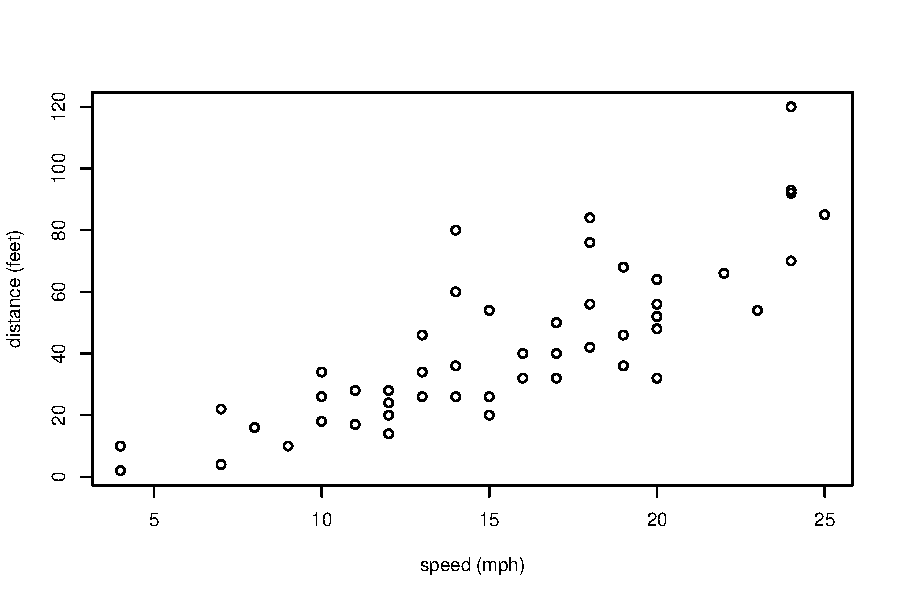
\includegraphics[width=\textwidth]{cars.pdf}
  \caption{This is my first figure. Figure captions should be located below
	the figure.}
  \label{fig:cars}
\end{figure}


\section{Discussion}
\label{sec:disc}

Answer the following questions in the Discussion (and Conclusion; see Note 5 for 
more details).

\begin{itemize}
\item What are the main contributions and key features or our analysis and results?
\item How did this research address the `need' identified in the introduction?
\item Do our results (appear to) confirm or contradict our initial expectations?
\item What are the generalizations and limitations of the current study?
\item What are our recommendations for our readers?
\item What are worth pursuing further in the future?
\end{itemize}


Note that we used \verb|enumerate| in Section~\ref{sec:intro} for a numbered 
list, but used \verb|itemize| above for a bulleted list.


Remember your project must integrate programming, data management,
data analysis, data visualization, and data ethics (collection and use).  
Make sure these are addressed in this document!


Optional Acknowledgements and Appendix sections are 
commented out below. Simply remove the $\%$ symbol in front of \verb|\section| 
and the corresponding section will be included.  
(The $*$ after \verb|\section| prevents these sections from being numbered in 
the document). 

Generally references should appear after acknowledgements, but before any
appendices. Be sure to check your bib entries for both formatting and 
completeness. 


\section*{Supplemental Materials}

Supplemental materials are separate files and document(s), so the purpose of 
this section is to describe the location and contents of the supplemental 
material.  

All code and data used in this manuscript are available at \url{my.github.page}.

Descriptions and results of additional supplemental analyses are provided in 
supplement.pdf, also available at \url{my.github.page}.


%\section*{Acknowledgements} %optional


\bibliography{refs}
\bibliographystyle{mcap}


%\section*{Appendix} %optional


\end{document}